% thanks to Jean-Julien Fleck who created this template : https://www.overleaf.com/latex/templates/presentation-beamer-pour-tipe-2019/jnrdxpgkwpbc

\documentclass{beamer}
\usepackage{currfile}
\usepackage{textcomp}
\usepackage{stmaryrd}
\usepackage{empheq}
\usepackage{algorithm}
\usepackage{algorithmicx}
\usepackage{color}
\usepackage{bbold}
\usepackage{mathtools}
\usepackage{pgfplotstable}
\usepackage{pgfplots}
\usepackage[export]{adjustbox}
\usepackage{siunitx}
\usepackage{hyperref}
\usepackage{caption}
\usepackage{subcaption}
\usepackage{minted}
\usepackage{tikz}     % Un package pour les dessins (utilisé pour l'environnement {code})
\usepackage[framemethod=TikZ]{mdframed}
\usepackage[T1]{fontenc}    % Encodage des accents
\usepackage[utf8]{inputenc} % Lui aussi
\usepackage[frenchb]{babel} % Pour la traduction française
\usepackage{numprint}       % Histoire que les chiffres soient bien

\usepackage{amsmath}        % La base pour les maths
\usepackage{mathrsfs}       % Quelques symboles supplémentaires
\usepackage{amssymb}        % encore des symboles.
\usepackage{amsfonts}       % Des fontes, eg pour \mathbb.

\usemintedstyle{friendly}
\pgfplotsset{compat=newest}
\pgfplotsset{every axis y label/.style={at={(yticklabel cs:1)},anchor=north east, rotate=90}}

\newcommand{\imagesource}[1]{{\footnotesize Source : #1}}

%%%%%%%%%%%%%%%%%%%%%%%%%%%%%%%%%%%%%%%%%
% Beamer Presentation
% LaTeX Template
% Version 1.0 (10/11/12)
%
% This template has been downloaded from:
% http://www.LaTeXTemplates.com
%
% License:
% CC BY-NC-SA 3.0 (http://creativecommons.org/licenses/by-nc-sa/3.0/)
%
%%%%%%%%%%%%%%%%%%%%%%%%%%%%%%%%%%%%%%%%%

%----------------------------------------------------------------------------------------
%	PACKAGES AND THEMES
%----------------------------------------------------------------------------------------




\mode<presentation> {

% The Beamer class comes with a number of default slide themes
% which change the colors and layouts of slides. Below this is a list
% of all the themes, uncomment each in turn to see what they look like.

%\usetheme{default}
%\usetheme{AnnArbor}
%\usetheme{Antibes}
%\usetheme{Bergen}
%\usetheme{Berkeley}
%\usetheme{Berlin}
%\usetheme{Boadilla}
%\usetheme{CambridgeUS}
%\usetheme{Copenhagen}
%\usetheme{Darmstadt}
%\usetheme{Dresden}
%\usetheme{Frankfurt}
%\usetheme{Goettingen}
%\usetheme{Hannover}
%\usetheme{Ilmenau}
%\usetheme{JuanLesPins}
%\usetheme{Luebeck}
\usetheme{Madrid}
%\usetheme{Malmoe}
%\usetheme{Marburg}
%\usetheme{Montpellier}
%\usetheme{PaloAlto}
%\usetheme{Pittsburgh}
%\usetheme{Rochester}
%\usetheme{Singapore}
%\usetheme{Szeged}

%\usetheme{Warsaw}

% As well as themes, the Beamer class has a number of color themes
% for any slide theme. Uncomment each of these in turn to see how it
% changes the colors of your current slide theme.

%\usecolortheme{albatross}

%\usecolortheme{beaver}

%\usecolortheme{beetle}
%\usecolortheme{crane}
%\usecolortheme{dolphin}
%\usecolortheme{dove}
%\usecolortheme{fly}
%\usecolortheme{lily}
%\usecolortheme{orchid}
%\usecolortheme{rose}
%\usecolortheme{seagull}

\usecolortheme{seahorse}

%\usecolortheme{whale}
%\usecolortheme{wolverine}

%\setbeamertemplate{footline} % To remove the footer line in all slides uncomment this line
%\setbeamertemplate{footline}[frame number] % To replace the footer line in all slides with a simple slide count uncomment this line

%\setbeamertemplate{navigation symbols}{} % To remove the navigation symbols from the bottom of all slides uncomment this line

\setbeamercovered{transparent} % Fait apparaître les animations en grisé (utile pour la conception, mais peut être commenté lors de la remise du document final)

% Pour utiliser une police à empattements partout
\usefonttheme{serif}



}

\usepackage{graphicx} % Allows including images
\usepackage{booktabs} % Allows the use of \toprule, \midrule and \bottomrule in tables



% Ce fichier contient toutes les macros que vous pouvez avoir envie de définir 
% si vous les utilisez plusieurs fois dans le document.

\PassOptionsToPackage{svgnames}{color}

% Un environnement pour bien présenter le code informatique
\newenvironment{code}{%
\begin{mdframed}[linecolor=green,innerrightmargin=30pt,innerleftmargin=30pt,
backgroundcolor=black!5,
skipabove=10pt,skipbelow=10pt,roundcorner=5pt,
splitbottomskip=6pt,splittopskip=12pt]
}{%
\end{mdframed}
}

% Un raccourci pour composer les unités correctement (en droit)
% Exemple: $v = 10\U{m.s^{-1}}$
\newcommand{\U}[1]{~\mathrm{#1}}

% Les guillemets \ofg{par exemple}
\newcommand{\ofg}[1]{\og{}#1\fg{}}

% Le d des dérivées doit être droit: \frac{\dd x}{\dd t}
\newcommand{\dd}{\text{d}}

% La dérivée temporelle, tellement courante en physique, avec les d droits
\newcommand{\ddt}[1]{\frac{\dd #1}{\dd t}}

% Des parenthèses, crochets et accolades qui s'adaptent automatiquement à la 
% taille de ce qu'il y a dedans
\newcommand{\pa}[1]{\left(#1\right)}
\newcommand{\pac}[1]{\left[#1\right]}
\newcommand{\paa}[1]{\left\{#1\right\}}

% Un raccourci pour écrire une constante
\newcommand{\cte}{\text{C}^{\text{te}}}

% Pour faire des indices en mode texte (comme les énergie potentielles)
\newcommand{\e}[1]{_{\text{#1}}}

% Le produit vectoriel a un nom bizarre:
\newcommand{\vectoriel}{\wedge}


\title[Mouvements de Foules]{TIPE : Modélisation d’une foule d’usagers du métro parisien}
\author{Louis \textsc{Thevenet}}
\institute[TIPE]{Épreuve de TIPE}
\date{Session 2023} 

\begin{document}
\begin{frame}
    \titlepage
\end{frame}

\begin{frame}
    \frametitle{Plan de l'exposé}
    \tableofcontents
\end{frame}

% Titre de la premiere partie
\section{Introduction Historique}

%%%%%%%%%%%%%%%%%%%%%%%%%%%%%%%%%%%%%%%%%%%%%%%%
% Première diapo
%%%%%%%%%%%%%%%%%%%%%%%%%%%%%%%%%%%%%%%%%%%%%%%%
\begin{frame}
\frametitle{Contexte scientifique }
\framesubtitle{Premiers modèles}

Craig Reynolds (1987) : Premier modèle de mouvement de foule : les boids


\begin{itemize}
	\item	<2->	Représentation de nuées d’oiseaux
	\item	<3->	Règles très simples
	\item   <4->      Vitesses et trajectoires des agents liées aux voisins proches

	\visible<5->{
	\begin{figure}
	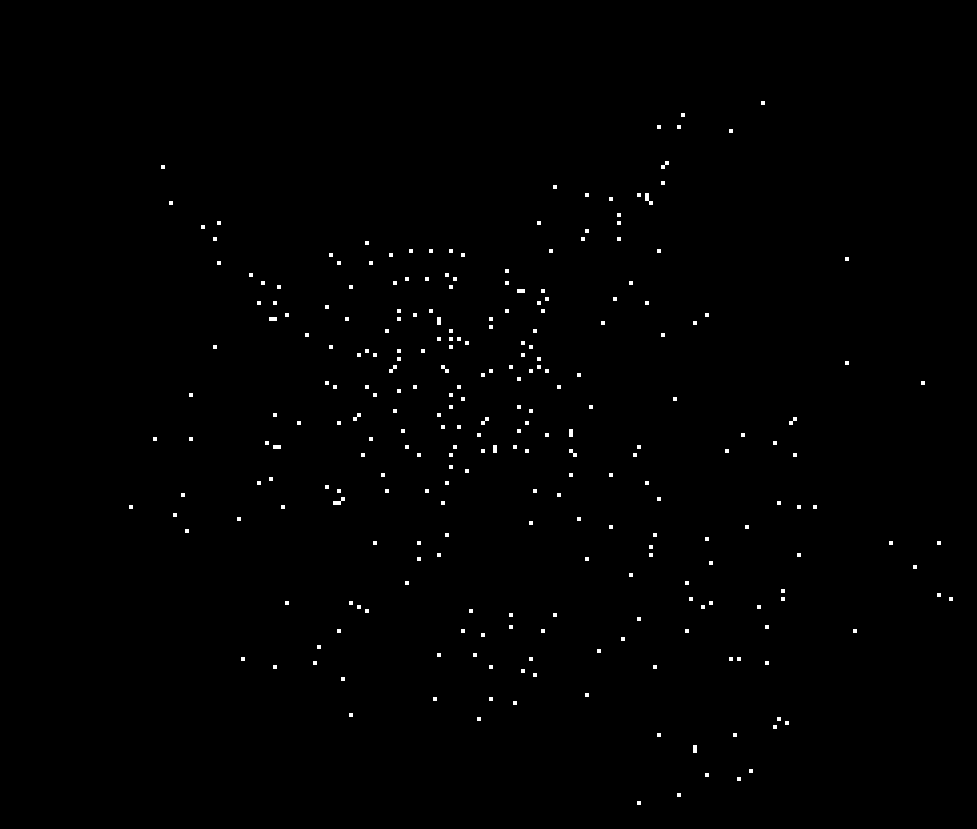
\includegraphics[width=0.5\linewidth]{figures/Fig01}
	\end{figure}
	}
	
\end{itemize}

\end{frame}


%%%%%%%%%%%%%%%%%%%%%%%%%%%%%%%%%%%%%%%%%%%%%%%%
% Deuxième diapo
%%%%%%%%%%%%%%%%%%%%%%%%%%%%%%%%%%%%%%%%%%%%%%%%
\begin{frame}
\frametitle{Introduction historique}
\framesubtitle{Premiers modèles}

% AFFICHAGE PAS TERRIBLE ICI
Dirk Helbing et Péter Molnar (1998) : Le concept de "forces sociales"


\begin{itemize}
	\item	<2->	Force d’attraction sociale : les trajectoires peuvent être influencées

	\item	<3->	Force de répulsion : les contacts physiques sont évités
 \end{itemize}
\bigskip
\onslide<4-> Julien Pettre et Wouter Van Toll (2021) : Evitement de collision

 \begin{itemize}
     \item <5-> Les trajectoires sont adoucies et plus réalistes en fonction des obstacles
 \end{itemize}	

\end{frame}


%%%%%%%%%%%%%%%%%%%%%%%%%%%%%%%%%%%%%%%%%%%%%%%%
% Troisième diapo
%%%%%%%%%%%%%%%%%%%%%%%%%%%%%%%%%%%%%%%%%%%%%%%%
%\begin{frame}
%\frametitle{Introduction historique}
%\framesubtitle{Modèles plus réalistes}
%
%Bertrand Maury/Juliette Venel (2009) : Modèle plus réaliste
%
%\begin{itemize}
%	\item	<1->	Agents représentés par des cercles (pas de chevauchement)
%    \item <2-> Forces de répulsion
%	\item	<3-> Prédiction de mouvement
%\end{itemize}
%\end{frame}


%%%%%%%%%%%%%%%%%%%%%%%%%%%%%%%%%%%%%%%%%%%%%%%%
% Quatrième diapo
%%%%%%%%%%%%%%%%%%%%%%%%%%%%%%%%%%%%%%%%%%%%%%%%
\begin{frame}
\frametitle{Introduction historique}
\framesubtitle{Modèles plus réalistes}


\visible<1->{
	\begin{figure}
	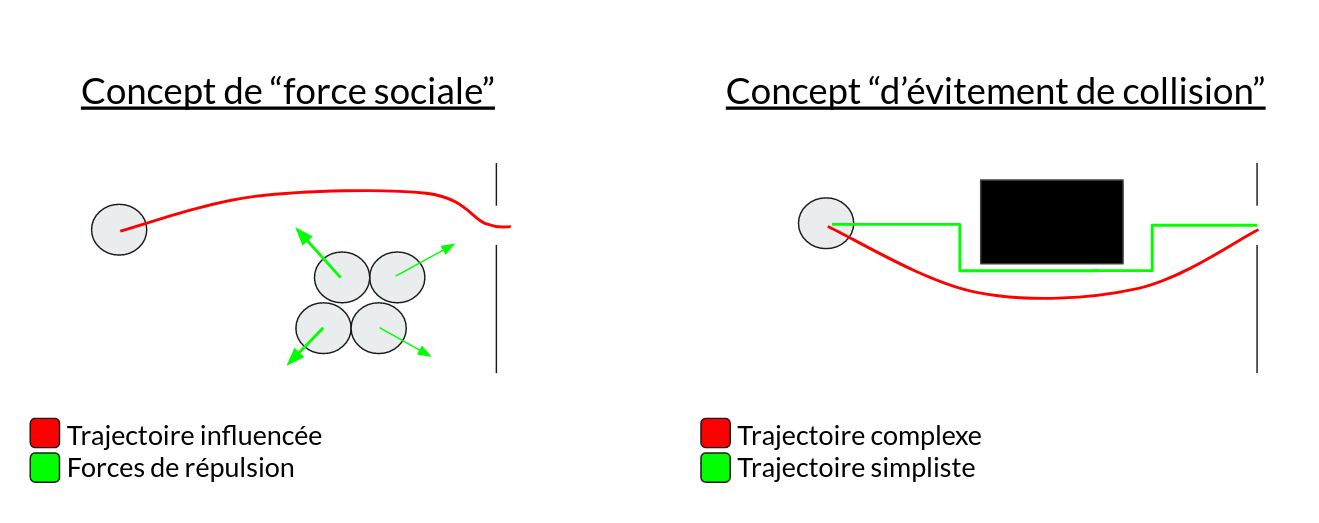
\includegraphics[width=1\linewidth]{figures/Fig02}
	\end{figure}
}
 
\end{frame}

\section{Problématisation}

\begin{frame}
    \frametitle{Problématique}
    \framesubtitle{Questions soulevées}

    \textbf{Problématisation}

    \begin{itemize}
        \item <2-> Quelles sont les lois essentielles qui permettent de décrire le mouvement d'une foule à l'échelle de l'individu ?
              \bigskip
        \item <3-> Comment implémenter une telle modélisation afin de vérifier la cohérence architecturale de lieux très fréquentés ?

    \end{itemize}
\end{frame}

% Le titre de la partie
\section{Construction du modèle}


%%%%%%%%%%%%%%%%%%
% Plan
%%%%%%%%%%%%%%%%%%

\begin{frame}
\frametitle{Modélisation}
\framesubtitle{Plan}
    \textbf{Modélisation}
    \begin{itemize}
        \item <2-> Modèle mathématique simple
        \item <3-> Adaptation informatique
        \item <4-> Amélioration du modèle
    \end{itemize}
\end{frame}


%%%%%%%%%%%%%%%%%%%%%%%%%%%%%%%%%%%%%%%%%%%%%%%%
% Première diapo
%%%%%%%%%%%%%%%%%%%%%%%%%%%%%%%%%%%%%%%%%%%%%%%%

\begin{frame}
\frametitle{Modèle mathématique}
\framesubtitle{Simplifications}

On restreint l’étude à deux dimensions, en \textbf{discrétisant} le temps et le plan :
\bigskip


\begin{itemize}
    \item <2-> Carte $\leftrightarrow P_{i,j} \in M_{n,p}(\mathbb{N}), (n, p) \in \mathbb{N}^2$
    \item <3->  Agent $ \leftrightarrow position, but \in \llbracket 1, n\rrbracket \times \llbracket 1, p\rrbracket $
\end{itemize}

\end{frame}


%%%%%%%%%%%%%%%%%%%%%%%%%%%%%%%%%%%%%%%%%%%%%%%%
% Deuxième diapo: le code informatique impose un 
% environnement "fragile" pour la frame
%%%%%%%%%%%%%%%%%%%%%%%%%%%%%%%%%%%%%%%%%%%%%%%%

\begin{frame}[fragile]
\frametitle{Modèle mathématique}
\framesubtitle{Implémentation des structures}

\begin{code}
\begin{minted}[linenos]{c}
struct location {
  int y;
  int x;
}

struct person {
  struct location pos;
  struct location goal;
}
\end{minted}
\end{code}
\end{frame}



%%%%%%%%%%%%%%%%%%%%%%%%%%%%%
% troisième diapo
%%%%%%%%%%%%%%%%%%%%%%%%%%%%%

\begin{frame}[fragile]
\frametitle{Modèle mathématique}
\framesubtitle{Implémentation des structures}


\begin{code}
\begin{minted}[linenos]{c}
struct map {
int **level;      // plan de la simulation
int start_nb;     // nombre d'entrées
location *starts; // et leurs positions
int exit_nb;      // nombre de sorties
location *exits;  // et leurs positions
int width;        // largeur
int height;       // hauteur
}
\end{minted}
\end{code}

\[ map \rightarrow level[i][j] \leftrightarrow \text{ nombre de personnes à la position } (i,j)\]
\end{frame}



%%%%%%%%%%%%%%%%%%%%%%%%%%%%%
% quatrième diapo
%%%%%%%%%%%%%%%%%%%%%%%%%%%%%

\begin{frame}
\frametitle{Modèle mathématique}
\framesubtitle{Squelette du programme}

On définit des fonctions :\\
\begin{itemize}
    \item Simulation
        \begin{itemize}
            \item <2-> $charger\_carte$
            \item <3-> $intention$
            \item <4-> $deplacement$
        \end{itemize}

\bigskip
    \item <5-> Génération des résultats
        \begin{itemize}
            \item <6-> $creer\_image$
            \item <7-> $sauvegarder\_image$
        \end{itemize}
\end{itemize}
\end{frame}



%%%%%%%%%%%%%%%%%%%%%%%%%%%%%
% cinquième diapo
%%%%%%%%%%%%%%%%%%%%%%%%%%%%%


\begin{frame}
\frametitle{Modèle mathématique}
\framesubtitle{Précisions}

Notant \(\mathbb{A}\) l'ensemble des agents de la simulation, $intention$ et $deplacement$ se définissent par :



\begin{empheq}[left=intention \colon \empheqlbrace]{align*}
    \mathbb{A} \to& \mathbb{N}^2\\
    x \mapsto& intention(x)
\end{empheq}

\begin{empheq}[left=deplacement \colon \empheqlbrace]{align*}
    M_{n,p}(\mathbb{N}) \times \mathbb{A} \to& M_{n,p}(\mathbb{N})\\
    (M, x) \mapsto& deplacement(M, x)
\end{empheq}

\end{frame}


\section{Implémentation du modèle}

\begin{frame}

    \frametitle{Implémentation}
    \framesubtitle{Plan}
    \textbf{Implémentation}
    \begin{itemize}
        \item <2-> Choix d'implémentation
        \item <3-> Construction de la matrice d'adjacence
        \item <4-> Implémentation des algorithmes
    \end{itemize}
\end{frame}


\begin{frame}
    \frametitle{Implémentation}
    \framesubtitle{Choix}
    Deux algorithmes connus de recherche du plus court chemin :
    \begin{itemize}
        \item <2-> Dijkstra
        \item <3-> $\text{A}^{*}$
    \end{itemize}
    \bigskip
    Ceux-ci sont basés sur l'étude d'un \textbf{graphe associé} au problème
\end{frame}


\begin{frame}
    \frametitle{Implémentation}
    \framesubtitle{Graphe associé}
    On définit le graphe associé à une carte $M$ par :
    \bigskip
    \begin{align*}
        \onslide<2-> G_M =         & (S, A)                                                           \\
        \onslide<3-> \text{ avec } & S = \{u \in M \colon u \text{ est une position valide}\},        \\
        \onslide<4->               & A = \{(u,\ v)\in S \colon u \text{ et } v \text{ sont voisins}\}
    \end{align*}

\end{frame}


\begin{frame}
    \frametitle{Implémentation}
    \framesubtitle{Matrice d'adjacence}

    Dans le programme, le graphe $G_M$ est représenté par une matrice d'adjacence $A_G$ définie par :

    \begin{align*}
        \onslide<2-> S & = \{0, 1, \dots, n \times p - 1 \}                                                                                        \\
        \bigskip
        \onslide<3->   & \forall (i,j)\in \llbracket 0, n-1\rrbracket \times \llbracket 0, p-1\rrbracket,\space A_{G_{i,j}} = \mathbb{1}_{A} (i,j)
    \end{align*}
\end{frame}


\begin{frame}
    \frametitle{Implémentation}
    \framesubtitle{Algorithme}
    Algorithme utilisé : \bigskip
    \textbf{A*}
    \begin{itemize}
        \item <2-> Approxime le plus court chemin à l'aide d'une heuristique
        \item <3-> Explore le graphe en estimant la pertinence de chaque nœud pour se rendre à l'objectif
    \end{itemize}
\end{frame}


\begin{frame}
    \frametitle{Implémentation}
    \framesubtitle{Heuristique}
    Une heuristique est une application de la forme :
    \onslide<2->{
        \begin{empheq}[left=h \colon \empheqlbrace]{align*}
            \mathbb{R}^2 \times \mathbb{R}^2 \times M_{n,p}(\mathbb{N}) \to& \mathbb{R}\\
            (pos, pos_{but}, M) \mapsto& h(pos, pos_{but}, M)
        \end{empheq}
    }
    \onslide<3->{
        Exemple : la norme euclidienne
        \begin{empheq}[left=h \colon \empheqlbrace]{align*}
            \mathbb{R}^2 \times \mathbb{R}^2 \times M_{n,p}(\mathbb{N}) \to& \mathbb{R}\\
            ((x,y), (x', y'), M) \mapsto& \sqrt{(x'-x)^2 + (y-y')^2}
        \end{empheq}
    }
\end{frame}


\begin{frame}
    \frametitle{Implémentation}
    \framesubtitle{Cadre des tests}
    \textbf{Cadre} : quai de métro à l'arrivée d'un train (partie supérieure) et disposant de plusieurs accès (partie inférieure) \\[.3cm]
    \onslide<2-> Une case correspond à \num{1}\si{\metre \squared}, avec une limite de 6 \si{personnes \per \metre \squared}
    \onslide<3->{
        \begin{figure}
            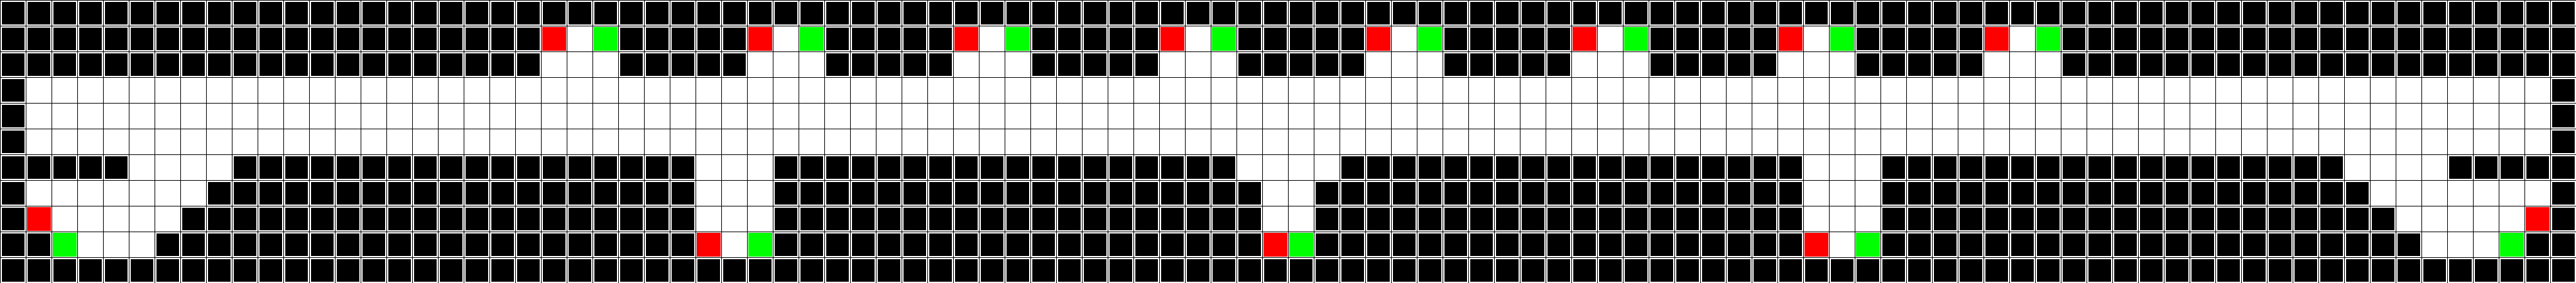
\includegraphics[width=1\textwidth]{figures/Fig05}
        \end{figure}
        \fcolorbox{black}{black}{\rule{0pt}{6pt}\rule{6pt}{0pt}}\quad Mur (case infranchissable) \\
        \fcolorbox{black}{white}{\rule{0pt}{6pt}\rule{6pt}{0pt}}\quad Quai (case franchissable) \\
        \fcolorbox{black}{green}{\rule{0pt}{6pt}\rule{6pt}{0pt}}\quad Sortie \\
        \fcolorbox{black}{red}{\rule{0pt}{6pt}\rule{6pt}{0pt}}\quad Entrée \\
    }
\end{frame}


\begin{frame}
    \frametitle{Implémentation}
    \framesubtitle{Test norme euclidienne}
    \textbf{Résultats du programme :} \\
    \onslide<2-> {Pour de petites populations initiales la simulation se \textbf{termine correctement} \\[.1cm]}
    \onslide<3->{Pour une population initiale de \textbf{600 agents}, la simulation n'aboutit pas à une évacuation complète :}
    \begin{figure}
        \only<3->{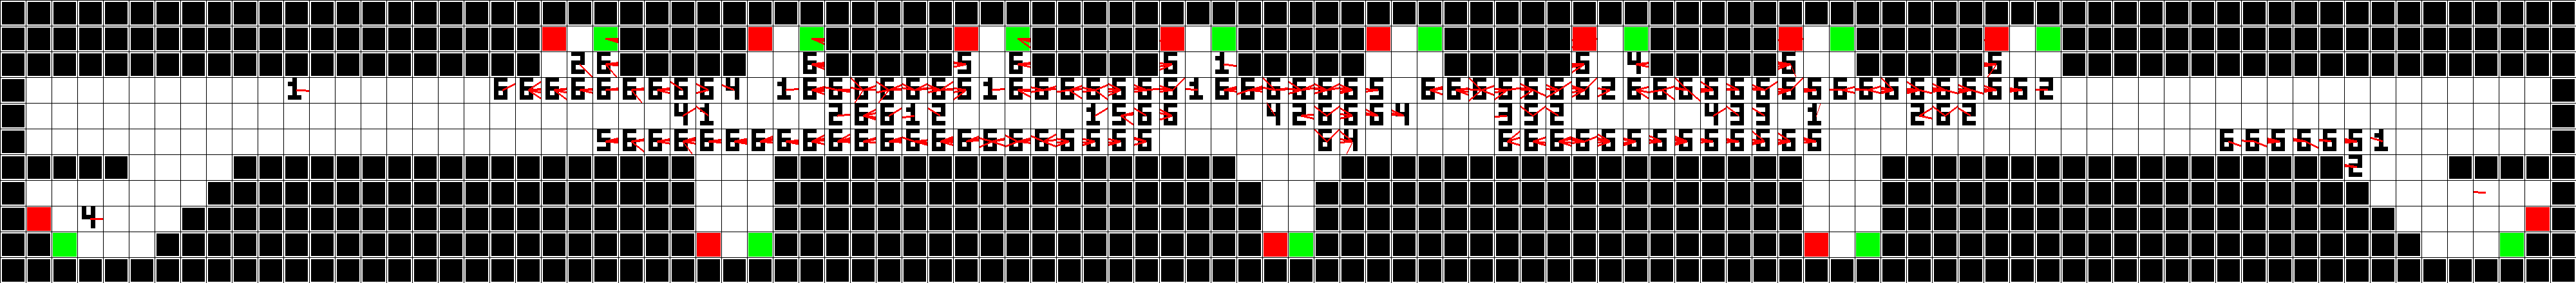
\includegraphics[width=1\textwidth]{figures/Fig03}\\[.5cm]}
        \begin{columns}
            \only<3->{
                \begin{column}{0.475\textwidth}
                    La simulation est \textbf{figée} de manière non réaliste : \\[.1cm]
                    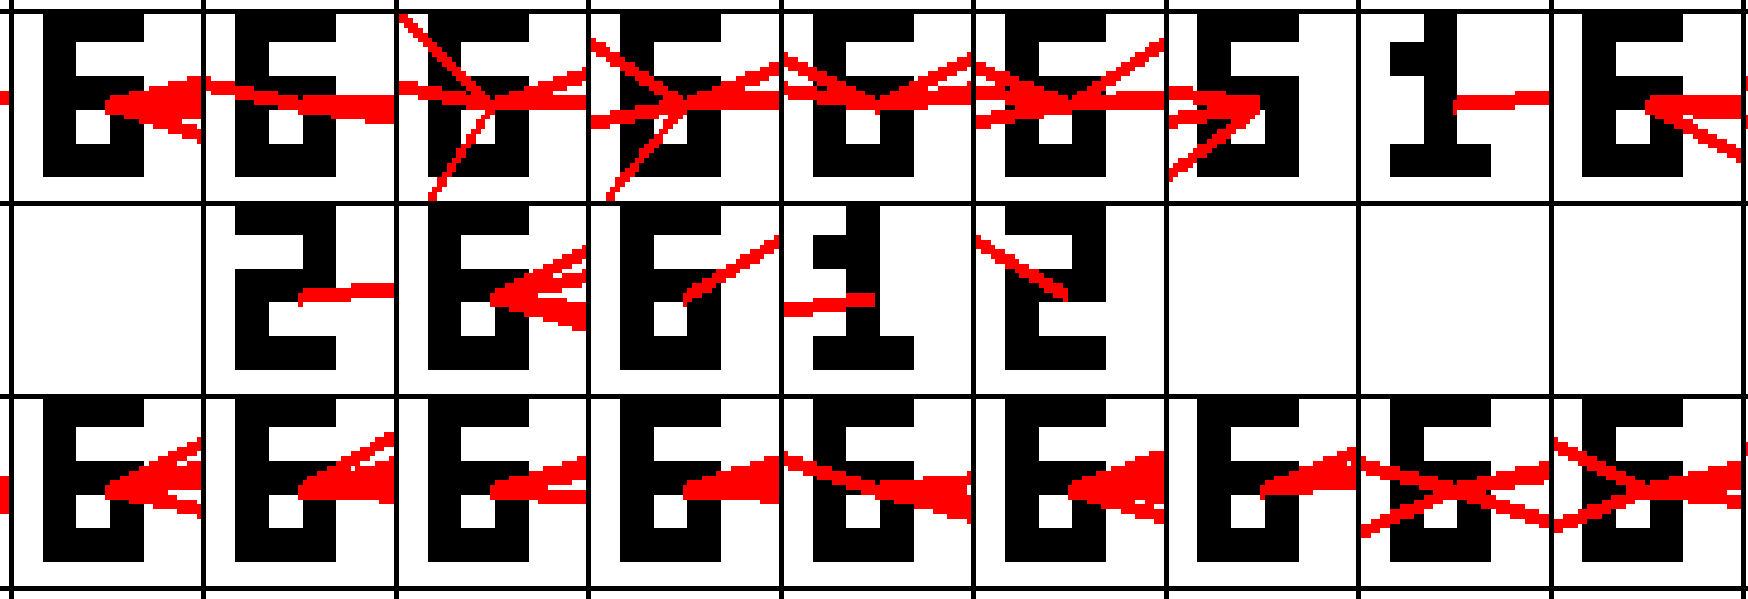
\includegraphics[width=.9\textwidth, left]{figures/Fig04}
                \end{column}
            }
            \only<4->{

                \begin{column}{.5\textwidth}
                    Cette heuristique n'est correcte que dans le cas d'un graphe constant. Or notre graphe varie en fonction des agents à proximité.
                \end{column}
            }
        \end{columns}
    \end{figure}
\end{frame}


\begin{frame}
    \frametitle{Implémentation}
    \framesubtitle{Une nouvelle heuristique}
    On cherche alors à modifier notre heuristique pour
    \begin{itemize}
        \item <2-> la rendre plus réaliste
        \item <3-> prendre en compte les agents à proximité
    \end{itemize}

\end{frame}


\begin{frame}[fragile]
    \frametitle{Implémentation}
    \framesubtitle{Proposition d'une heuristique}
    On ajoute pour cela un paramètre \textit{REPULSION} à la simulation :
    \begin{onslide}<2->
        \begin{code}
            \begin{minted}[linenos]{c}
int h(location pos, location goal, map *m) {
    int f = 1;
    for (int i=0; i<REPULSION; i++) {
        f*=m->level[pos.y][pos.x];
    }
    return f
           + (goal.x - pos.x) * (goal.x - pos.x)
           + (goal.y - pos.y) * (goal.y - pos.y);
}
    \end{minted}
        \end{code}
        Après avoir testé différentes valeurs, on a estimé que la valeur \textbf{4} renvoyait un résultat convenable.
    \end{onslide}


\end{frame}


\begin{frame}
    \frametitle{Implémentation}
    \framesubtitle{Test de cette nouvelle heuristique}
    \textbf{Résultats du programme :} \\
    \onslide<2->{Pour une population initiale de \textbf{600 agents}, la simulation ne rencontre plus de blocage.\\[.2cm]}
    \onslide<3->{Le nouveau blocage est rencontré pour des populations initiales \textbf{supérieures à 1000 agents.}}
    \begin{figure}
        \onslide<4->{
            Le mouvement est maintenant limité par l'agencement même du lieu :\\[.1cm]}
        \only<4>{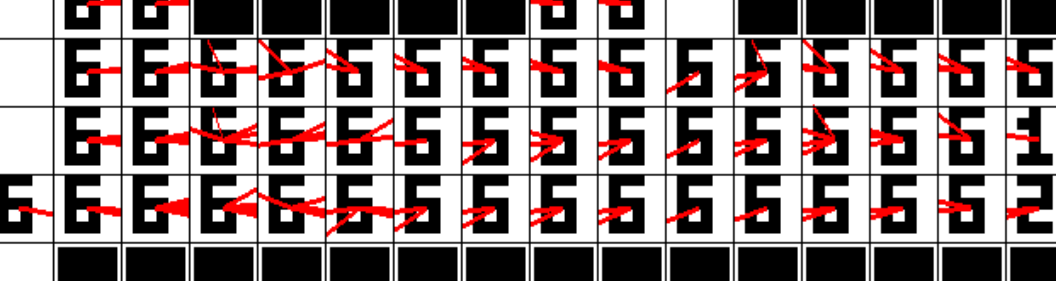
\includegraphics[scale=0.3]{figures/Fig06}}
    \end{figure}
\end{frame}


\begin{frame}
    \frametitle{Implémentation}
    \framesubtitle{Déplacements plus réaliste}
    On cherche maintenant à obtenir un déplacement plus réaliste en introduisant des limites de densité : \\
    \begin{itemize}
        \item <2-> Densité acceptable : 3 p/m²
        \item <3-> Densité maximale : 6 p/m²
    \end{itemize}
    \bigskip
    \onslide<4->{Si la case visée contient N agents, le déplacement est possible si :}
    \begin{itemize}
        \item <5-> $N<3$
        \item <6-> $2 <N< 6$ et l'agent subit des pressions extérieures de la part d'au moins deux agents
    \end{itemize}
\end{frame}


\begin{frame}
    \frametitle{Implémentation}
    \framesubtitle{Résultats de cette nouvelle fonction}
    La nouvelle fonction permet un déplacement plus réaliste des agents qui s'éparpillent dans l'espace après être entrés dans la pièce. \\[.1cm]
    \begin{figure}
        \centering
        \begin{subfigure}{.5\textwidth}
            \centering
            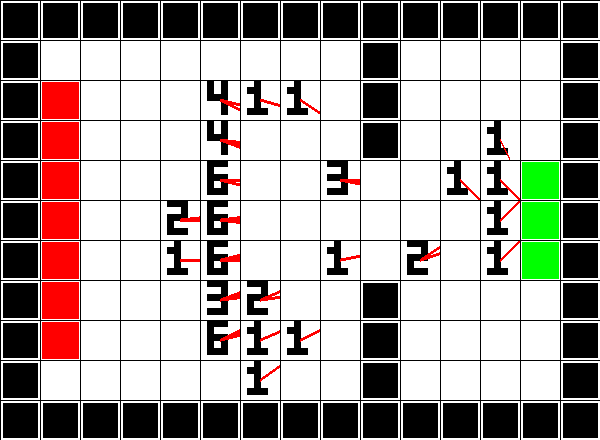
\includegraphics[scale=0.2]{figures/Fig10}\caption{Ancienne fonction}
            \label{fig:sub1}
        \end{subfigure}%
        \begin{subfigure}{.5\textwidth}
            \centering
            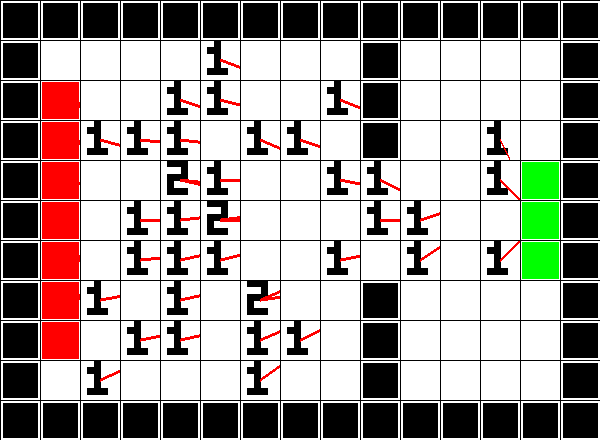
\includegraphics[scale=0.2]{figures/Fig11}
            \caption{Nouvelle fonction}
            \label{fig:sub2}
        \end{subfigure}
        \label{fig:test}
    \end{figure}
    \tiny{
        \fcolorbox{black}{green}{\rule{0pt}{6pt}\rule{6pt}{0pt}}\quad Sortie \
        \fcolorbox{black}{black}{\rule{0pt}{6pt}\rule{6pt}{0pt}}\quad Mur (case infranchissable)\\
        \fcolorbox{black}{red}{\rule{0pt}{6pt}\rule{6pt}{0pt}}\quad Entrée
        \fcolorbox{black}{white}{\rule{0pt}{6pt}\rule{6pt}{0pt}}\quad Air (case franchissable)
    }
\end{frame}
\section{Applications du modèle}

\begin{frame}
    \frametitle{Applications}
    \framesubtitle{Plan}
    \textbf{Deux applications du programme}\\
    \begin{itemize}
        \item <2-> Evaluation du trafic maximal d'un quai de métro
        \item <3-> Vérification de résultats scientifiques connus
    \end{itemize}
\end{frame}


\begin{frame}
    \frametitle{Evaluation du trafic maximal}
    \framesubtitle{Cadre des tests}
    \textbf{Cadre} : quai de métro à l'arrivée d'un train \\[.3cm]
    \begin{figure}
        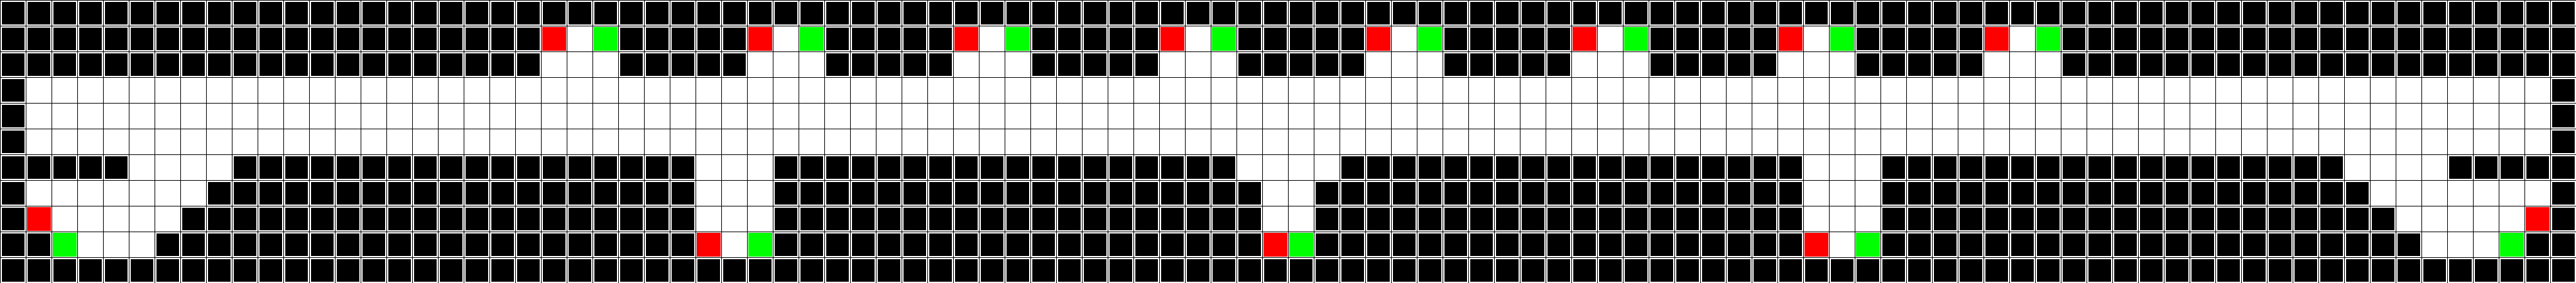
\includegraphics[width=1\textwidth]{figures/Fig05}
    \end{figure}
    \begin{columns}
        \begin{column}{0.35\textwidth}
            \tiny{\fcolorbox{black}{black}{\rule{0pt}{6pt}\rule{6pt}{0pt}}\quad Mur (case infranchissable) \\
                \fcolorbox{black}{white}{\rule{0pt}{6pt}\rule{6pt}{0pt}}\quad Quai (case franchissable) \\
                \fcolorbox{black}{green}{\rule{0pt}{6pt}\rule{6pt}{0pt}}\quad Sortie \\
                \fcolorbox{black}{red}{\rule{0pt}{6pt}\rule{6pt}{0pt}}\quad Entrée \\}
        \end{column}
        \begin{column}{0.7\textwidth}
            \onslide<2-> Longueur du quai : \num{100} \si{\metre} \\
            \onslide<3-> Largeur du quai : \num{3} \si{\metre}  \\
            \bigskip
            \onslide<4-> Surface de la partie centrale : $50 \times 3 = 150$ \si{\metre \squared}   \\[.5cm]
            \onslide<5-> Ainsi, le quai est dimensionné pour recevoir
            \begin{itemize}
                \item <6-> dans un cas normal : $150 \times 3 = 450$ usagers
                \item <7-> dans un cas critique : $150 \times 6 = 900$ usagers
            \end{itemize}
        \end{column}
    \end{columns}
\end{frame}


\begin{frame}
    \frametitle{Evaluation du trafic maximal}
    \framesubtitle{Protocole de test}
    \textbf{Protocole de test}
    \begin{itemize}
        \item <2-> relève du nombre d'étapes de simulation pour une population initiale donnée
        \item <3-> moyenne sur 20 mesures pour chaque point
        \item <4-> relève du nombre de simulations qui n'ont pas terminé pour chaque population initiale
    \end{itemize}
\end{frame}


\begin{frame}
    \frametitle{Evaluation du trafic maximal}
    \framesubtitle{Variation de la population initiale}
    \begin{tikzpicture}
        \begin{axis}[width=1\textwidth,height=.8\textheight,xlabel=Population initiale,ylabel=Etapes, legend style={at={(0.45,0.05)},anchor=south west},]
            \addplot table [y=temps, x=population]{data/pop_etapes_heuristique.txt};
            \addplot [red, mark = x, nodes near coords=2,every node near coord/.style={anchor=-90}] coordinates {( 1000, 148)};
            \addplot [red, mark = x, nodes near coords=5,every node near coord/.style={anchor=-90}] coordinates {( 1050, 151)};
            \addplot [red, mark = x, nodes near coords=1,every node near coord/.style={anchor=-90}] coordinates {( 950, 146)};
            \addplot [red, mark = x, nodes near coords=10,every node near coord/.style={anchor=+90}] coordinates {( 1100, 150)};
            \addplot [red, mark = x, nodes near coords=13,every node near coord/.style={anchor=-90}] coordinates {( 1150, 161)};
            \addplot [red, mark = x, nodes near coords=19,every node near coord/.style={anchor=+90}] coordinates {( 1200, 173)};
            \addplot [red, mark = x, nodes near coords=20,every node near coord/.style={anchor=+90}] coordinates {( 1250, 501)};
            \addplot [red, mark = x, nodes near coords=20,every node near coord/.style={anchor=-90}] coordinates {( 1300, 501)};
            \addplot [red, mark = x, nodes near coords=20,every node near coord/.style={anchor=+90}] coordinates {( 1350, 501)};
            \draw[dashed][black] (-100, 501) -- node[below] {limite fixée} (1600, 501);
            \legend{itérations par pop. initiale, simulations qui se figent};
        \end{axis}
        \node[align=center,font=\bfseries, yshift=1em] (title)
        at (current bounding box.north)
        {Durée de simulation pour une population initiale donnée};
    \end{tikzpicture}
\end{frame}


\begin{frame}
    \frametitle{Evaluation du trafic maximal}
    \framesubtitle{Conclusion}
    \begin{tikzpicture}
        \begin{axis}[width=1\textwidth,width=1\textwidth, height=.4\textheight,xlabel=Population initiale,legend style={at={(0.45,0.05)},anchor=south west},]
            \addplot table [y=temps, x=population]{data/pop_etapes_heuristique.txt};
            \addplot [red, mark = x, nodes near coords=1,every node near coord/.style={anchor=-90}] coordinates {( 950, 146)};
            \addplot [red, mark = x, nodes near coords=2,every node near coord/.style={anchor=-90}] coordinates {( 1000, 148)};
            \addplot [red, mark = x, nodes near coords=5,every node near coord/.style={anchor=-90}] coordinates {( 1050, 151)};
            \addplot [red, mark = x, nodes near coords=10,every node near coord/.style={anchor=+90}] coordinates {( 1100, 150)};
            \addplot [red, mark = x, nodes near coords=13,every node near coord/.style={anchor=-90}] coordinates {( 1150, 161)};
            \addplot [red, mark = x, nodes near coords=19,every node near coord/.style={anchor=+90}] coordinates {( 1200, 173)};
            \addplot [red, mark = x, nodes near coords=20,every node near coord/.style={anchor=+90}] coordinates {( 1250, 501)};
            \addplot [red, mark = x, nodes near coords=20,every node near coord/.style={anchor=-90}] coordinates {( 1300, 501)};
            \addplot [red, mark = x, nodes near coords=20,every node near coord/.style={anchor=+90}] coordinates {( 1350, 501)};
            \draw[dashed][black] (-100, 501) -- node[below] {limite fixée} (1600, 501);
        \end{axis}
        \node[align=center,font=\bfseries, yshift=1em] (title)
        at (current bounding box.north)
        {Durée de simulation pour une population initiale donnée};
    \end{tikzpicture}
    \onslide<2-> On retrouve bien des blocages à partir d'une population initiale d'environ 950 personnes. \\[.5cm]
    \onslide<3-> Le modèle renvoie bien un résultat cohérent avec la valeur estimée.
\end{frame}


\begin{frame}
    \frametitle{Divsion du flux}
    \framesubtitle{Présentation du phénomène}
    \textbf{Placement d'un obstacle devant une sortie} \\
    Ce phénomène s'interprète comme une division du flux incident
    \begin{columns}
        \begin{column}{0.475\textwidth}
            \begin{figure}
                Illustration
                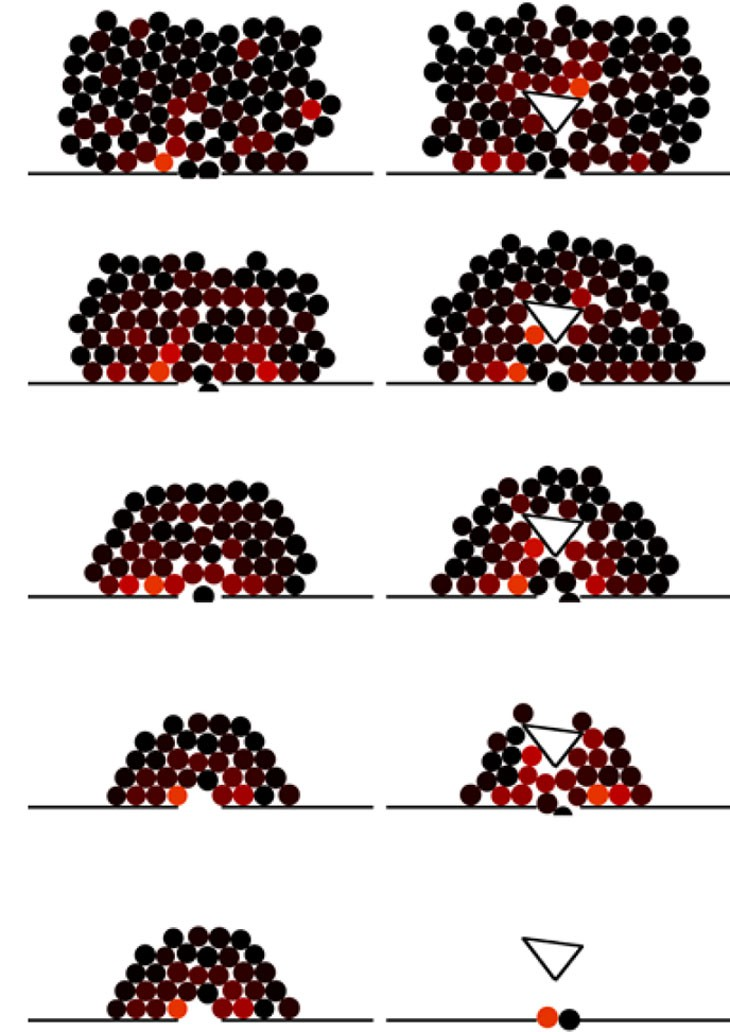
\includegraphics[height=.58\textheight]{figures/Fig07}
                \imagesource{\href{https://www.pourlascience.fr/sd/mathematiques/la-foule-en-equations-17252.php}{Pour La Science N°501}}
            \end{figure}
        \end{column}
        \only<2>{\begin{column}{0.475\textwidth}
                \begin{figure}
                    On souhaite mettre en valeur ce phénomène : \\[.2cm]
                    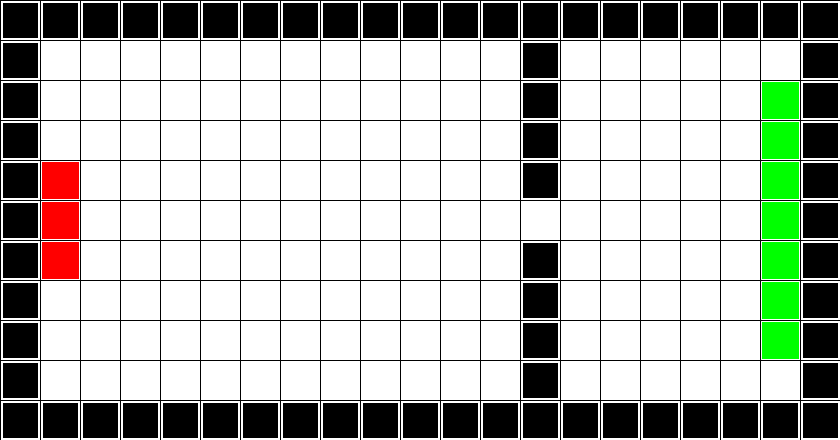
\includegraphics[width=.6 \textwidth]{figures/Fig09} \\[.3cm]
                    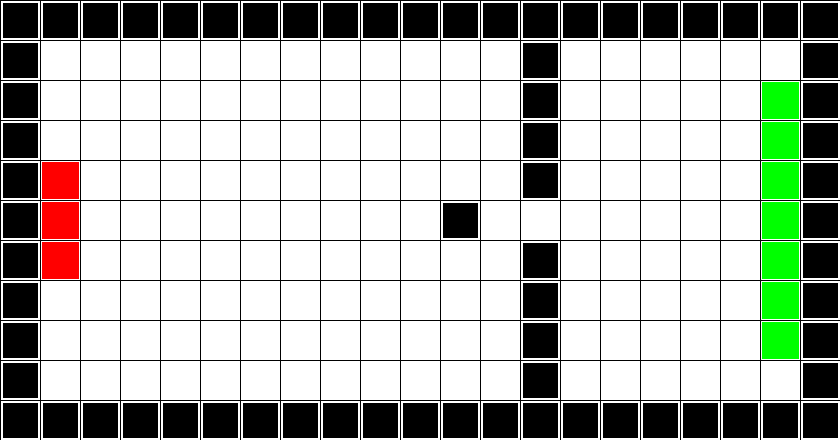
\includegraphics[width=.6\textwidth]{figures/Fig08}
                \end{figure}
            \end{column}
        }
    \end{columns}
\end{frame}


\begin{frame}
    \frametitle{Division du flux}
    \framesubtitle{Protocole de test}
    \textbf{Protocole de test}
    \begin{itemize}
        \item <2-> relève du nombre d'étapes de simulation pour une population initiale donnée
        \item <3-> relève du nombre de cases pour lesquelles la densité a dépassé 5 personnes/m²
        \item <4-> moyenne sur 50 mesures pour chaque point
    \end{itemize}
\end{frame}


\begin{frame}
    \frametitle{Division du flux}
    \framesubtitle{Résultats du programme}
    \begin{tikzpicture}
        \begin{axis}[width=1\textwidth,height=.8\textheight,xlabel=Population,ylabel=étapes\ \ \ , legend style={at={(0.05,0.95)},anchor=north west},]
            \addplot table [blue, y=temps, x=population]{data/pop_sans_obstacle.txt};
            \addplot table [red, y=temps, x=population]{data/pop_avec_obstacle.txt};
            \only<2->{\addplot table [blue, y=dens, x=population]{data/pop_sans_obstacle.txt};
                \addplot table [red, y= dens, x=population]{data/pop_avec_obstacle.txt};}
            \tiny{\legend{durée sans obstacle, durée avec obstacle, occurences de densités $\geq 5$ p/m² sans obstacle, occurences de densités $\geq 5$ p/m² avec obstacle}};
        \end{axis}
        \node[align=center,font=\bfseries, yshift=1em] (title)
        at (current bounding box.north)
        {Durée de simulation pour une population initiale donnée};
    \end{tikzpicture}
\end{frame}


\begin{frame}
    \frametitle{Division du flux}
    \framesubtitle{Conclusion}
    \begin{tikzpicture}
        \begin{axis}[width=1\textwidth,height=.4\textheight,xlabel=Population,legend style={at={(0.05,0.95)},anchor=north west},]
            \addplot table [blue, y=temps, x=population]{data/pop_sans_obstacle.txt};
            \addplot table [red, y=temps, x=population]{data/pop_avec_obstacle.txt};
            \addplot table [blue, y=dens, x=population]{data/pop_sans_obstacle.txt};
            \addplot table [red, y= dens, x=population]{data/pop_avec_obstacle.txt};
        \end{axis}
        \node[align=center,font=\bfseries, yshift=1em] (title)
        at (current bounding box.north)
        {Durée de simulation pour une population initiale donnée};
    \end{tikzpicture}
    On constate une évacuation plus rapide avec l'obstacle ainsi qu'un nombre moins important de situations dangereuses pour les agents. \\[1cm]
    Le modèle renvoie bien un résultat en accord avec le phénomène décrit.
\end{frame}


\begin{frame}
    \frametitle{Conclusion}
    La modélisation informatique de foules a de nombreuses applications :\\
    \begin{itemize}
        \item <2-> Sécurité et dimensionnement des infrastructures
        \item <3-> Etude de comportement sociaux
        \item <4-> Cinéma, jeux vidéo
    \end{itemize}
    \bigskip
    \bigskip
    \huge{Merci de votre attention.}
\end{frame}
%! Author = louis
%! Date = 05/06/23

% Le titre de la partie
\section{Annexe}

%%%%%%%%%%%%%%%%%%%%%%%%%%%%%%%%%%%%%%%%%%%%%%%%
% Première diapo
%%%%%%%%%%%%%%%%%%%%%%%%%%%%%%%%%%%%%%%%%%%%%%%%

\begin{frame}



\title{Annexe : programme}
    \maketitle

\end{frame}

\begin{frame}[
    t, % align text from top
    allowframebreaks, % allow brake frames
    fragile % allow verb content
]{map.c}
    \frametitle{map.c}
    \scriptsize
    \inputminted[breaklines,breakanywhere]{c}{../../map.c}
\end{frame}

\begin{frame}[
    t, % align text from top
    allowframebreaks, % allow brake frames
    fragile % allow verb content
]{person.c}
    \frametitle{person.c}
    \scriptsize
    \inputminted[breaklines,breakanywhere]{c}{../../person.c}
\end{frame}


\begin{frame}[
    t, % align text from top
    allowframebreaks, % allow brake frames
    fragile % allow verb content
]{min\_heap.c}
    \frametitle{min\_heap.c}
    \scriptsize
    \inputminted[breaklines,breakanywhere]{c}{../../min_heap.c}
\end{frame}

\begin{frame}[
    t, % align text from top
    allowframebreaks, % allow brake frames
    fragile % allow verb content
]{move.c}
    \frametitle{move.c}
    \scriptsize
    \inputminted[breaklines,breakanywhere]{c}{../../move.c}
\end{frame}


\begin{frame}[
    t, % align text from top
    allowframebreaks, % allow brake frames
    fragile % allow verb content
]{image.c}
    \frametitle{image.c}
    \scriptsize
    \inputminted[breaklines,breakanywhere]{c}{../../image.c}
\end{frame}




\begin{frame}[
    t, % align text from top
    allowframebreaks, % allow brake frames
    fragile % allow verb content
]{main.c}
    \frametitle{main.c}
    \scriptsize
    \inputminted[breaklines,breakanywhere]{c}{../../main.c}
\end{frame}
\end{document}
